\section{MongoDB}
\subsection{Visitenkarte} 
MongoDB ist ein schemaloses NoSQL Datenbanksystem, welches auf Dokumentenspeicherung setzt. Es ist in C++ programmiert\cite{Boicea01} und speichert die Dokumente in einem JSON \"ahnlichen Format, was BSON(Binary JSON) genannt wird. MongoDB wurde im Jahre 2010 zum ersten Mal f\"ur die breite Masse ver\"offentlicht und wurde zuletzt Ende November 2016 auf der Version 3.4 geupdated.\cite{mongo01}
\subsubsection{Geschichte}
MongoDB wurde von Dwight Merriman, Eliot Horowitz und seinem Team erstellt. Doch dies nicht auf direktem Wege. 2007 plante das MongoDB Team ein Onlineservice f\"ur Web-Anwendungen. Dieser Service sollte die M\"oglichkeit bieten, eine Web-Anwendung zu entwickeln, zu hosten und zu skalieren. Aufgrund von einem nicht geeigneten Datenbanksystem entschloss sich das Team ein eigenes Datenbanksystem zu erstellen und zu nutzen. Diese hatte noch keinen Namen, da dieses System speziell f\"ur den Service des Teams erstellt wurde. Im Jahre 2008 wurde dann das Datenbanksystem fertiggestellt. 2009 entschloss sich das Team, dieses Datenbanksystem, was sie erstellt haben, als Open Source Produkt freizugeben. Dieses System wurde als MongoDB ver\"offentlicht. M\"arz 2010 kam die erste Version von MongoDB heraus, die man in einem gr\"o\"sseren Umfang verwenden kann. \"Uber die Jahre wurde MongoDB von dem Team weiterentwickelt und ist zurzeit mit der Version 3.2 ver\"offentlicht.\cite{Shakuntala01}
\subsubsection{Anwendungsf\"alle}
MongoDB wird von verschiedenen Unternehmen zu verschiedensten Anwendungen und Aufgaben verwendet.
MTV verwendet MongoDB als Haupt-repository f\"ur das MTV-Network.
SourceForge verwendet MongoDB als Back-End Speicher.
Bit.ly verwendet MongoDB, um den Verlauf von Nutzern zu speichern.
New York Times verwendet MongoDB  f\"ur eine Foto-Abgabe.\cite{Boicea01}
\subsubsection{Besonderheiten}
MongoDB ist ein Datenbanksystem, was darauf ausgelegt wurde, schnell und Flexible mit einer guten Skalierung. Die Entwickler von MongoDB haben MongoDB nicht als die beste Datenbankl\"osung entwickelt, sondern als ein System, was f\"ur F\"alle wie komplexe Datensammlungen geeignet ist. Zudem stellt das MongoDB Team eine umfangreiche Dokumentation mit vielen Beispielen und Erkl\"arungen f\"ur jede ver\"offentlichte Version von MongoDB. MongoDB kann keine SQL-Befehle direkt ausf\"uhren, besitzt aber Funktionen, die die Funktionen von SQL \"ubernehmen wie ORDER BY und DISTINCT.
\subsubsection{Grenzen}
MongoDB besitzt in mehrere Bereiche Limitationen, die die Performance und das Nutzen von MongoDB einschr\"anken. 
\begin{itemize}
\item 32bit Version von MongoDB kann nur eine Datenbank einrichten, die maximal 2 GB gro\"ss sein kann. Dieses Problem kann behoben werden, indem man die 64bit Version von MongoDB verwendet. Zudem wird die 32bit Version von MongoDB nicht mehr seit der 3.0 Version unterst\"utzt.
\item BSON Dokumente k\"onnen maximal 16MB gro\"ss sein, was aber in Vergleich zu anderen Datenbanksystemen sehr gro\"ss ist.
\item Indexe in MongoDB k\"onnen nicht gr\"o\"sser als 1024 Byte sein. Zudem kann eine Collection maximal 64 Indexe besitzen. Auch der Name des Indexes ist auf 128 Byte begrenzt. Diese Limitationen sollten bei einer gut aufgebauten Datenbank nicht erreicht werden.
\item Das Sharding sollte wenn m\"oglich so fr\"uh wie m\"oglich eingef\"uhrt werden, da sonst die Performance von MongoDB stark beeintr\"achtigt wird, da die Server die Daten auf den unterschiedlichen Shards verteilen muss. Zudem sollte auch geachtet werden, das die Datenbank nicht \"uber 256 GB gro\"ss ist, da MongoDB bei einer Gr\"o\"sse von 256 GB das Sharding nicht mehr erlaubt.
\item Die Daten die bei MongoDB versendet werden sind nicht verschl\"usselt.
Bei Lese und Schreibvorg\"ange bei der MongoDB muss man auf Gro\"ss- und Kleinschreibung achten, da MongoDB Case-Sensitive ist.
\item MongoDB besitzt keine JOIN-Operation. Man muss diese durch verschachtelte Dokumente oder auf einen Verweis auf das jeweilige Dokument machen.
\end{itemize}
\subsection{Systemtechnologie}
\subsubsection{Referenzierung}
Die Referenzierung von MongoDB unterscheidet sich von der Referenzierung von den relationalen Datenbanken. Eine M\"oglichkeit der Referenzierung in MongoDB w\"are die Verschachtlung, also ein Dokument in einem Dokument schreiben. Damit kann man die Referenz auf ein anderes Objekt direkt erkennen, was auch f\"ur das System einfacher ist, an diese Daten zu gelangen. Das Problem hierbei kann aber eine zu starke Verschachtelungsstruktur sein, was auf Kosten der \"Ubersichtlichkeit geht, zus\"atzlich wird f\"ur ein Dokument mehr Platz gebraucht, da in einem Dokument ein weiteres existiert. Die zweite M\"oglichkeit f\"ur eine Referenzierung, w\"are der Verweis auf das jeweilige Dokument. Das verbessert die \"Ubersicht und man kann erkennen, voraus die Daten herkommen. Ein Problem was MongoDB mit sich bringt, ist, dass es keine Direktreferenzierung gibt. In der Relationalen Datenbank kann man mit dem JOIN Befehl die Referenz zu einem anderen Datensatz in Bezug auf einen anderen Datensatz direkt ansprechen und anzeigen lassen. Dies kann MongoDB nicht. Um dies zu erm\"oglichen, muss man das in einer eigenen Applikation programmieren.\cite{mongo01}
\subsubsection{Replikation}
Eine Replikation bei MongoDB ist die Kopie von Daten auf weiteren Servern. Dies nennt man replica set. Ein replica set umfasst Server mit derselben Funktionalit\"at und Dient zur Stabilisierung der Aufgabe des jeweiligen replica sets. Die MongoDB Website empfiehlt das Verwenden von drei Servern pro replica set, um somit die Ausfallrate gering zu halten. Die Daten in einem replica set sind auf allen Servern identisch. MongoDB verwendet das Master-Slave System f\"ur die Replikation von Daten innerhalb des replica sets. In dem replica set gibt es genau einen Primary und beliebig viele Secondary Server und ggf. einen Arbiter. Daten\"anderungen wie z.B. Schreiboperationen werden auf dem Primary Server in dem replica set durchgef\"uhrt. Nachdem die Operation erfolgreich beendet wurde, \"ubernehmen die Secondary Server die \"Anderung von dem Primary Server. Sollte der Primary Server ausfallen, so w\"ahlen die Secondary Server einen neuen Primary Server aus. Man ist in der Lage, in dem replica set einen Arbiter hinzuzuf\"ugen. Ein Arbiter besitzt nicht die Daten, die in dem replica set verteilt werden. Der Arbiter dient lediglich dazu, nur bei einer Abstimmung eine Stimme abzugeben, damit eventuelle Probleme bei einer Abstimmung vermieden werden k\"onnen. Ein Arbiter selber kann nicht zu einem Primary oder Secondary Server ernannt werden.\cite{mongo01}
\\
\\
\begin{minipage}{\textwidth}
    \centering
    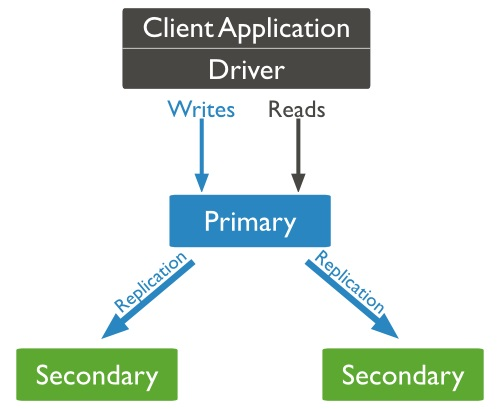
\includegraphics[scale=0.3]{images/01_replica-set-read-write-operations-primary.jpg}
    \captionof{figure}{Replikationsaufbau von MongoDB von \cite{mongo01}}
    \label{fig:ver}
\end{minipage}
\subsubsection{Indexierung}
Indizes in MongoDB dienen zur verbesserten Ausf\"uhrung von Abfragen. Durch Indizies  \"uberpr\"uft MongoDB nicht alle Dokumenten innerhalb einer Collection, sondern nur die Dokumente, die mit dem abgefragten Index versehen ist. Ohne Indizes w\"urde MongoDB immer die Collection komplett nach dem Abfragekriterium \"uberpr\"ufen. Ein Index, was MongoDB bei jeden Dokument automatisch erstellt, ist der id Index. Dieser dient dazu, jedes Dokument mit einem eindeutigen Wert zu versehen, das nur auf dieses Dokument zugewiesen werden kann, also wie ein Prim\"arschl\"ussel in relationalen Datenbanken. Um Indizes zu erstellen, wird folgender Befehl verwendet:
\\
\\
db.collection.createIndex()
\\
\\
Innerhalb der Klammern kann bestimmt werden, welcher Wert als Index gew\"ahlt werden soll und welche Art von Index verwendet wird. Indizes sind an einer Collection gebunden und k\"onnen auch nur in dieser verwendet werden. Wenn man ein Index erstellt, sollte darauf geachtet werden, dass der gew\"ahlte Wert nicht bereits ein Index besitzt.  Ebenso sollte darauf geachtet werden, dass m\"oglichst viele Dokumente den Wert besitzen, der indexiert wird.\cite{mongo01}
MongoDB bietet viele verschiedene Arten von Indizes an, die verwendet werden k\"onnen.
\begin{itemize}
\item Single Field Index die sich nur auf ein Wert beziehen
\item Compound Index, womit man ein Index mit mehreren Werten bestimmen kann
\item Multikey Index mit einem Wert, der aus mehreren Werten besteht
\item Geospatial Index f\"ur Geometrische Werte
\item Text Indexes um Werte mit Texten zu indexieren
\item Hashed Indexes f\"ur Hash basierte Verteilung
\end{itemize}
Zudem kann man indizes mit Eigenschaften versehen:
\begin{itemize}
\item Unique Indexes sind Indizes, die nur einmalige Werte akzeptiert
\item Partial Indexes sind Indizes nach bestimmten Filteroptionen
\item Sparse Indexes indexiert nur die Dokumente, die den angegebenen Wert besitzen
\item TTL Indexes sind Indizes, die die indexierte Werte nach einer angegebenen Zeit automatisch l\"oscht.
\end{itemize}
\subsubsection{Sharding}
MongoDB ist in der Lage, Daten \"uber mehreren Servern zu verteilen. Diese Methode wird Sharding genannt. Sharding ist in der Lage, in einem Cluster von Servern Daten von einer Datenbank aufzuteilen, sodass dadurch das Abrufen der Daten verbessert und beschleunigt wird. Ein sharded cluster besteht aus drei Komponenten: Den Config Server, den Query Server und Shards. Um ein sharded cluster einzurichten, braucht man mindestens einen Config Server, einen Query Server und 2 Shards. Dies sieht dann wie folgt aus:
\\
\\
\begin{minipage}{\textwidth}
    \centering
    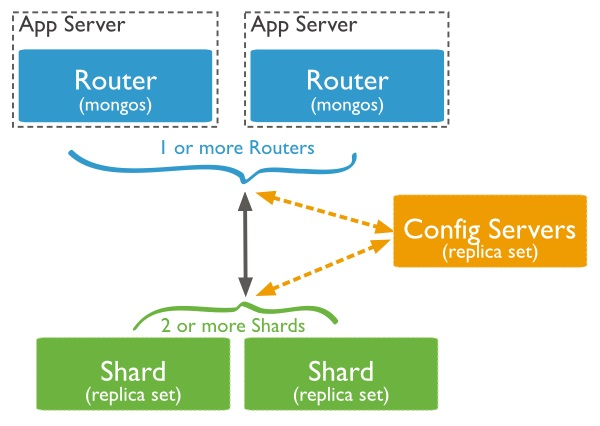
\includegraphics[scale=0.3]{images/01_sharded-cluster-production-architecture.jpg}
    \captionof{figure}{Aufbau vom Cluster Sharding in MongoDB von \cite{mongo01}}
    \label{fig:ver}
\end{minipage}
\\
\\
Config Server: Der Config Server in einem sharded Cluster beinhaltet die Metadaten f\"ur dieses. Diese Metadaten beinhalten die Informationen zu der Organisation und die Zust\"ande der jeweiligen Komponenten in dem sharded Cluster.  Ein Config Server ist in einem replica set. Ein replica set verbessert die Konsistenz \"uber die verschiedenen Config Server. Zus\"atzlich kann man danke dem replica set mehr als 3 Config Server nutzen.
Query Server (Router): Mit dem Query Server ist man in der Lage, Daten auf den verschiedenen Shards zu schreiben und zu Lesen. Dies vollbringt er mit den Metadaten, die der Query Server von dem Config Server bekommt. Der Query Server ist die einzige Schnittstelle in dem sharded Cluster, womit man auf die Daten durch Anwendungen zugreifen kann. 
\\
\\
\begin{minipage}{\textwidth}
    \centering
    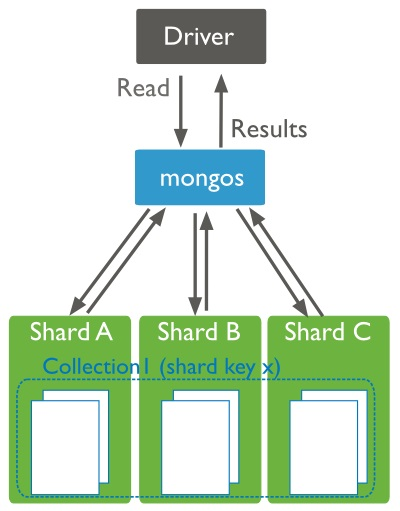
\includegraphics[scale=0.3]{images/01_sharded-cluster-scatter-gather-query.jpg}
    \captionof{figure}{Datenverteilung von dem Query Server von \cite{mongo01}}
    \label{fig:ver}
\end{minipage}
\\
\\
Shard: Bei einer Shard handelt es sich um einen Teil der Gesamtdatenbank. Die Daten, die in die Datenbank eingetragen werden, werden nach den Metadaten des Configservers analysiert und dann durch den Query Server auf das jeweilige Shard gespeichert. Zum Beispiel: Eine 3 Shard Datenbank beinhaltet Daten von Personen in einem Unternehmen. Auf Shard 1 werden alle Mitarbeiter gespeichert, die im Nachnamen mit dem Buchstaben A bis H anfangen. Shard 2 hat den Nachnamen von I bis Q und Shard 3 R bis Z. Dadurch, dass die Daten aufgeteilt und auf unterschiedlichen Shards gespeichert werden, ist man in der Lage schneller an die gew\"unschten Informationen zu kommen. Shards k\"onnen sich in einem replica set befinden. Dieses dient f\"ur Redundanz  und hohe Verf\"ugbarkeit der Daten.\cite{mongo01}
\subsection{Datenmodell}
Allgemeiner Aufbau von MongoDB
MongoDB ist ein dokumentenbasiertes schemaloses Datenbanksystem. Daten werden dementsprechend in Dokumenten gespeichert. Eine MongoDB-Datenbank besteht aus einer oder mehreren Collections. Und Jede Collection besitzt mindestens ein oder mehrere Dokumente. 
\\
\\
\begin{minipage}{\textwidth}
    \centering
    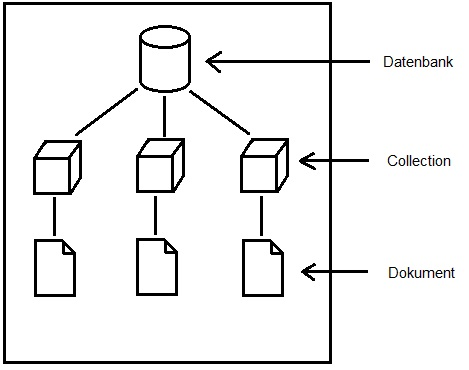
\includegraphics[scale=0.3]{images/01_Datenmodell_Mongo.jpg}
    \captionof{figure}{Datenbankstruktur von MongoDB nachkonstruiert nach \cite{mongo01}}
    \label{fig:ver}
\end{minipage}
\\
\\
Collections in MongoDB besitzen keine Vorgaben, wie ein Dokument aufgebaut sein sollte. So ist man in der Lage, jede Art von Dokument in Collections einzuf\"ugen. Dies sollte aber vermieden werden, da dadurch das Abfragen von den Dokumenten verkompliziert wird. Dokumente in MongoDB k\"onnen bis zu 16 MB gro\"ss sein. So ist es m\"oglich, eine gro\"sse Menge an Daten in ein einziges Dokument zu speichern, was aber auf Kosten der \"Ubersicht und der Performance geht.
\subsection{Systeminstallation}
\subsubsection{Installation von MongoDB}
Da uns Linux Ubuntu 16.04 Server zur Verf\"ugung stehen f\"ur die Installation von MongoDB, m\"ussen wir dementsprechend MongoDB f\"ur Linux Ubuntu 16.04 installieren. MongoDB muss auf allen Nodes in dem Cluster installiert werden. Es wurde MongoDB 3.2 installiert, da diese zum Zeitpunkt der Installation die aktuellste Version von MongoDB war. Zurzeit gibt es MongoDB in der Version 3.4. Dementsprechend richtet sich die Installation und Konfiguration von MongoDB auf die Version 3.2
\\
Um MongoDB auf Ubuntu zu installieren, m\"ussen folgede Schritte durchgef\"uhrt werden.
\\
\\
1.	Um bei Ubuntu mit apt oder dpkg MongoDB zu installieren, wird ein Public key ben\"otigt. Diesen bekommt man durch folgenden Befehl:
\\
\\
sudo apt-key adv --keyserver hkp://keyserver.ubuntu.com:80 --recv EA312927
\\
\\
2.	Danach muss eine Listendatei f\"ur MongoDB erstellt werden. Diese muss die Version, die installiert wird im Namen beinhalten. Der hier verwendete Befehl lautet:
\\
\\
sudo tee /etc/apt/sources.list.d/mongodb-org-3.2.list
\\
\\
3.	Bevor man MongoDB installiert, sollte der Ubuntu Server und deren Applikationen aktualisiert werden mit dem Befehl:
\\
\\
sudo apt-get update
\\
\\
4.	Nachdem nun alle Vorbereitungen getroffen worden sind, kann man nun MongoDB installieren. Der Befehl hierf\"ur lautet wie folgt:
\\
\\
sudo apt-get install -y mongodb-org
\\
\\
Nachdem MongoDB installiert wurde, was einige Minuten in Anspruche nehmen kann, kann man nun MongoDB starten. Und das mit dem Befehl: 
\\
\\
sudo service mongod start
\\
\\
Jetzt da der Mongod Service gestartet wurde, k\"onnen wir nun unsere Beispieldatenbank erstellen. MongoDB erstellt automatisch eine Datenbank, sollte diese bef\"ullt werden mit Dokumenten. Um die Beispieldatenbank zu erstellen, m\"ussen wir diese erst mit dem “Use“ Befehl von MongoDB ausw\"ahlen. Da wir unsere Datenbank abDB nennen, so lautet der “Use“ Befehl:
\\
\\
use abDB
\\
\\
Nun k\"onnen wir mit ``db.createCollection()`` eine Collection f\"ur unsere Beispieldatenbank erstellen. Der ganze Befehl denn wir verwendet haben lautet:
\\
\\
db.createCollection(‚abDBsimpleCSV‘,{capped:true,size:1024,max:3000})
\\
\\
Jetzt wird die Datenbank in MongoDB auch abgespeichert. Wie die Daten von der Datenbank auf unsere Beispieldatenbank \"ubertragen werden, wird in Kapitel 4.1.1 n\"aher erl\"autert.
\\
Nun da wir MongoDB auf unserem Cluster auf jedem Node gestartet und eine Datenbank angelegt wurde, k\"onnen wir nun die Konfiguration von MongoDB f\"ur das Sharding vornehmen.\cite{mongo01}
\subsubsection{Konfiguration von dem Sharding}
Wie schon im Kapitel 3.1.2 erl\"autert, braucht man f\"ur das Sharding einen Query-Server, mind. einen Replica Set an Config-Servern und mind. zwei Shards. Um das Sharding f\"ur MongoDB zu erm\"oglichen, muss man zuerst den Replica Set von dem Config Server vornehmen.
\\
\\
Konfiguration Config-Server Replica Set
\\
\\
Da ein Replica Set aus mind. 3 Servern bestehen muss, verwenden wir auch 3 Server um die Stabilit\"at der Server zu gew\"ahrleisten. Wir installieren die Config Server auf Node 1, 2 und 3. Die Vorgehensweise sieht wie folgt aus:
\\
\\
1.	Verzeichnisse f\"ur Dateien und Logs vom Config Server erstellen
\\
\\
sudo mkdir -p /db/config/log
\\
sudo mkdir -p /db/config/data
\\
\\
2.	Nun muss der Config Server gestartet werden:
\\
\\
sudo mongod --port 27022 --dbpath /db/config/data --configsvr --replSet abDBcs --fork --logpath /db/config/log/mongodb.log
\\
\\
Dieser Befehl muss bei allen Config Servern durchgef\"uhrt werden, und alle m\"ussen demselben Replica Set zugewiesen werden.
\\
\\
3.	Nachdem alle Config Server gestartet wurden, muss nun das Replica Set f\"ur die Config Server konfiguriert werden. Dazu m\"ussen wir zuerst in die Mongo Shell gehen. Mit der Mongo Shell ist man in der Lage, die Mongo Instanz zu bedienen. Die Mongo Shell startet man mit: 
\\
\\
mongo localhost:27022
\\
\\
In der Mongo Shell selber kann man dann das Replica Set konfigurieren. Dieser Befehl muss nur auf einen der Config Servern durchgef\"uhrt werden:
\\
\\
rs.initiate( \\
\{ \\
    \_id: “abDBcs“, \\
    configsvr: true, \\
    members: [ \\
      \{ \_id : 0, host : “10.20.110.43:27022“ \}, \\
      \{ \_id : 1, host : “10.20.110.41:27022“ \}, \\
      \{ \_id : 2, host : “10.20.110.39:27022“ \} \\
    ] \\
  \} \\
) \\
\\
Nun sollte in dem Replica Set ein Primary und die Secondarys ausgew\"ahlt werden. Damit sollte nun der Config Server Replica Set f\"ur das Sharding bereit sein.
\\
Nun werden die Shards konfiguriert. Die Shards werden fast genauso wie die Config Server konfiguriert. Shard 1 wird auf Node 1, 3 und 4 installiert und sieht wie folgt aus:
\\
\\
1.	Verzeichnisse f\"ur Dateien und Logs vom Shard 1 erstellen:
\\
\\
sudo mkdir -p /db/shard1/log
\\
sudo mkdir -p /db/shard1/data
\\
\\
2.	Nun m\"ussen die Server in dem Shard gestartet werden:
\\
\\
sudo mongod --port 27023 --dbpath /db/shard1/data --shardsvr --replSet abDBrs1 --fork --logpath /db/shard1/log/mongodb.log
\\
\\
3.	Wie auch bei dem Config Server muss nun mit der Mongo Shell auf einen der Servern das Replica Set eingestellt werden:
\\
\\
rs.initiate( \\
  \{ \\
  \_id: “abDBrs1“, \\
    members: [ \\
      \{ \_id : 0, host : “10.20.110.43:27023“ \}, \\
      \{ \_id : 1, host : “10.20.110.39:27023“ \}, \\
      \{ \_id : 2, host : “10.20.110.48:27023“ \} \\
    ] \\
  \} \\
) \\
\\
Shard 2 wird genauso installiert, nur das Shard 2 auf Node 2,3 und 4 installiert wird und ein eigenes Replica Set besitzt.
\\
\\
Nun muss der Query Server eingerichtet werden. Um den Query Server einrichten zu k\"onnen, m\"ussen die Shards bereits eingerichtet sein. Die Schritte f\"ur die Einrichtung von dem Query Server sehen wie folgt aus:
\\
\\
1.	Verzeichnis f\"ur die Log Dateien erstellen:
\\
\\
sudo mkdir -p /db/query/log
\\
\\
2.	Nun muss der Query Server gestartet werden. Hierbei ist es wichtig anzugeben, wo sich der Config Server befindet, da der Query Server die Meta Daten von dem Config Server ben\"otigt, um das Sharding auszuf\"uhren:
\\
\\
sudo mongos --configdb abDBcs/10.20.110.43:27022,10.20.110.41:27022,10.20.110.39:27022 --port 27021 --fork --logpath /db/query/log/mongodb.log
\\
\\
3.	Nachdem der Query Server gestartet wurde, m\"ussen nun die Shards mit der Mongo Shell dem Query Server zugeteilt werden, hierbei muss jeder einzelne Server von einem Shard eingetragen werden:
\\
\\
sh.addShard(“abDBrs1/10.20.110.43:27023“) \\
sh.addShard(“abDBrs1/10.20.110.39:27023“) \\
sh.addShard(“abDBrs1/10.20.110.48:27023“) \\
\\
sh.addShard(“abDBrs2/10.20.110.41:27024“) \\
sh.addShard(“abDBrs2/10.20.110.39:27024“) \\
sh.addShard(“abDBrs2/10.20.110.48:27024“) \\
\\
4.	Zum Schluss muss man dem Query Server sagen, welche Datenbank auf den Shards geteilt werden soll:
\\
\\
sh.enableSharding(“abDB“)
\\
\\
Nun wurde MongoDB auf Ubuntu installiert und das Sharding f\"ur die Datenbank ``abDB`` eingerichtet.\cite{mongo01}
\subsection{Datenschema}
Uns wurde eine CSV Datei bereitgestellt, die von dem Schema der relationellen Abschlussarbeitendatenbank entnommen wurde. Da die \"Ubername von dem relationellen Schema in MongoDB wenig Sinn ergibt, haben wir das Schema angepasst, damit es besser und effektiver von MongoDB verwaltet werden kann. Zuerst stellt sich die Frage: Wie viele Collections verwenden wir, um die Daten der Abschlussarbeitendatenbank in MongoDB darstellen zu k\"onnen. Wir haben uns dazu entschlossen, dass wir die Abschlussarbeitendatenbank in nur einer einzigen Collection abspeichern werden. Die Gr\"unde f\"ur diese Entscheidung lauten wie folgt:
\\
MongoDB verf\"ugt \"uber keine direkte Referenzierung auf andere Dokumente und Collections. Man kann diese zwar nennen in einem Dokument, man muss dann dieses Dokument mit einer weiteren Abfrage heraussuchen. Zudem sind Schemalose Datenbanksysteme darauf aufgebaut, gr\"o\"ssere Datenmengen aufzurufen.\cite{mongo01}
\\
Es ist einfacher Indizes auf einer gro\"ssen Collection durchzuf\"uhren. Indizes k\"onnen die Abfragezeit um das 10-fache verk\"urzen.
\\
Die Datenmenge die wir erhalten haben ist gering, sodass eine Aufteilung auf mehrere Collections nur mehr Aufwand als Hilfe darstellen w\"urde.
\subsection{Ad-Hoc-Zugriffsm\"oglichkeiten}
Um mit MongoDB Daten einzuf\"ugen oder auszulesen, sind verschiedene CRUD-Operationen notwendig, wie bei einer relationellen Datenbank. Diese Operationen \"ahneln wie JavaScript Anweisungen und sind daher leicht anzuwenden. Die wichtigsten Befehle zur Verwendung von MongoDB sind in Tabelle 2.1 zu entnehmen.\cite{mongo01}
\\
\\
\begin{table}[h]
\centering
\begin{tabular}{|p{7cm}|p{7cm}|c|c|}
\hline 
Befehl & Funktion \\ 
\hline 
Use <Datenbankname> & Setzt die Datenbank zu den benutzten Namen \\ 
\hline 
db.createCollection(„Name“,{capped : true, size : <byte>, max : <anzahl> }) & Legt eine Collection mit dem angegebenen Namen \\ 
\hline 
db.<name>.insert({Name: „Thomas“, Alter: 25, …})  & Legt ein Dokument in der Collection <name> ab \\ 
\hline 
db.<name>.save({Name: „Thomas“, Alter: 22}) & Einfache Veränderung eines Dokumentes mit dem Namen “Thomas” \\ 
\hline 
db.<name>.update({Name: „Thomas“}, {Name: „Franz“ , Alter: 24}) & Veränderung eines Dokumentes mit dem Namen „Thomas“ \\ 
\hline 
db.<name>.find() & Zeigt alle Dokumente in der Collection <name> \\ 
\hline 
db.<name>.count({Name: „Franz“}) & Zählt alle Dokumente, die den Namen “Franz” beinhalten \\ 
\hline 
db.<name>.remove({Name: “Franz”}) & Löscht alle Dokumente mit dem Namen “Franz” \\ 
\hline 
db.<name>.drop() & Die Collection löschen \\ 
\hline 
\end{tabular}
\caption{Befehlsliste für MongoDB}
\end{table} 
\\
Beim Arbeiten von MongoDB sollte stets geachtet werden, dass man auf der richtigen Datenbank arbeitet und dass die Dokumente in die richtige Collections eingetragen werden. Zudem sollte man auf Gro\"ss-  und Kleinschreibung achten, da MongoDB Case-Sensitive ist.